\documentclass{beamer}

\usepackage[utf8]{inputenc}
\usepackage[T1]{fontenc}
\usepackage{graphicx}
\usepackage{listings}
\usepackage{xcolor}

\useinnertheme{uconn}
\useoutertheme[]{uconn}
%\useoutertheme[footline=authorinstitute,subsection=true]{miniframes}
%\useoutertheme{sidebar}
\usecolortheme{default}
\usefonttheme{default}

\title[IntroToTensorflow]{Introduction to Tensorflow for NFL Sports Analytics}
\author[Pranav]{Pranav Tavildar}
\institute[UConn]{UConn Sports Analytics Symposium 2022}
\date{\today}

\setlength{\parskip}{.5em}

\lstdefinestyle{Python}{
    language        = Python,
    basicstyle      = \tiny,
    keywordstyle    = \color{blue},
    keywordstyle    = [2] \color{teal}, % just to check that it works
    stringstyle     = \color{green},
    commentstyle    = \color{red}\ttfamily
}


\begin{document}

\lstset{
    frame       = single,
    numbers     = left,
    showspaces  = false,
    showstringspaces    = false,
}

\begin{frame}
\titlepage
\end{frame}


\begin{frame}{Table of contents}
\tableofcontents
\end{frame}

\section{Introduction to Tensorflow}

\begin{frame}[fragile]{What is Tensorflow?}

  \begin{columns}[T]
    \begin{column}{.5\textwidth}
     \begin{block}{Open Source Deep Learning Library that makes creating Models more:}
     \begin{itemize}
     % Your text here
     \item Easy
     \item Flexible
     \item Fast
     \item Reproducable
    \end{itemize}
    \end{block}
    \end{column}
    \begin{column}{.5\textwidth}
    \begin{block}{}
% Your image included here
    {
\includegraphics[width=4cm]{images/tflogo.png}}
    \end{block}
    \end{column}
  \end{columns}

\end{frame}


\begin{frame}[fragile]{The History of Tensorflow}

  \begin{columns}[T]
    \begin{column}{.5\textwidth}
     \begin{block}{Evolution of Tensorflow}
     \begin{itemize}
     % Your text here
     \item Product of Google Brain Team
     \item Evolution from Distbelief (2011)
     \item Possible because of Tensor Processing Unit
    \end{itemize}
    \end{block}
    \end{column}
    \begin{column}{.5\textwidth}
    \begin{block}{}
% Your image included here
    {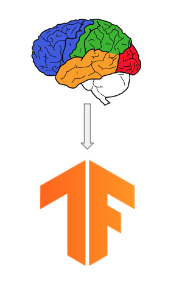
\includegraphics[width=3cm]{images/evolution.png}}
    \end{block}
    \end{column}
  \end{columns}

\end{frame}

%%%%%%%%%%%%%%%%%%
\begin{frame}[fragile]{Tensorflow vs Alternatives}
\begin{columns}[T]
 \begin{column}{.33\textwidth}
     \begin{block}{Tensorflow}
     \begin{itemize}
     \item Preferred by Companies
     \item Easily Deployable and Versatile
    \end{itemize}
     \end{block}
   \end{column}
   
    \begin{column}{.33\textwidth}
     \begin{block}{Pytorch}
     \begin{itemize}
     \item Preferred by Research Labs
     \item Easily Debuggable
    \end{itemize}
     \end{block}
   \end{column}
   
   \begin{column}{.33\textwidth}
     \begin{block}{Caffe}
     \begin{itemize}
     \item Used by Researchers and Startups
     \item Useful for Small but Specific and fast use cases
    \end{itemize}
     \end{block}
   \end{column}

\end{columns}
\end{frame}

\begin{frame}[fragile]{What is a Tensor?}
\begin{itemize}
	\item Tensor is data with dimension.
	\item 0-d tensor: scalar
	\begin{equation*}
	c = 5
	\end{equation*} 
	\item 1-d tensor: vector
	\begin{equation*}
	{\rm{c}} = \left( {\begin{array}{*{20}{c}}
1\\
 \vdots \\
5
\end{array}} \right)
	\end{equation*} 
	\item 2-d tensor: matrix
	\begin{equation*}
	{\rm{c}} = \left( {\begin{array}{*{20}{c}}
1& \cdots &5\\
 \vdots & \ddots & \vdots \\
5& \cdots &5
\end{array}} \right)
	\end{equation*}
\end{itemize}
\end{frame}


\begin{frame}[fragile]{Why Use Tensors?}
\begin{itemize}
	\item Vector, matrix operations and gradient (derivative) are dominant in machine learning and deep learning.
	\item GPU structure leads to a powerful ability to solve linear tensor operations.
\end{itemize}
\end{frame}


\begin{frame}[fragile]{How to install Tensorflow Locally}
\begin{itemize}
	\item Anaconda management (GUI): click "environment" --> choose "Not installed" --> search "tensorflow"
	\item Anaconda Prompt: 
	\begin{verbatim}
    conda install tensorflow
	\end{verbatim}
	\item Pip:
	\begin{verbatim}
    pip install tensorflow 
	\end{verbatim} 
	\item Verify whether your installation is successful: (open jupyter notebook or run at .py file)
	\begin{lstlisting}[style = Python]
import tensorflow as tf
import tensorflow.compat.v1 as tfv1
tf.__version__
\end{lstlisting}
\end{itemize}
\end{frame}

\section{Concepts and Basis}

\begin{frame}[fragile]{3 key concepts in tensorflow programming}
\begin{itemize}
	\item Operations: Data operations like "matmul" (matrix multiplication), "add".
	\item Graph: Build GRAPH which represents the data flow of the computation.
	\item Session: Run SESSION which executes the operations on the graph.
\end{itemize}
\uncover<2->
{
	\begin{picture}(0,0)(0,0)
		\put(90,-80)
		{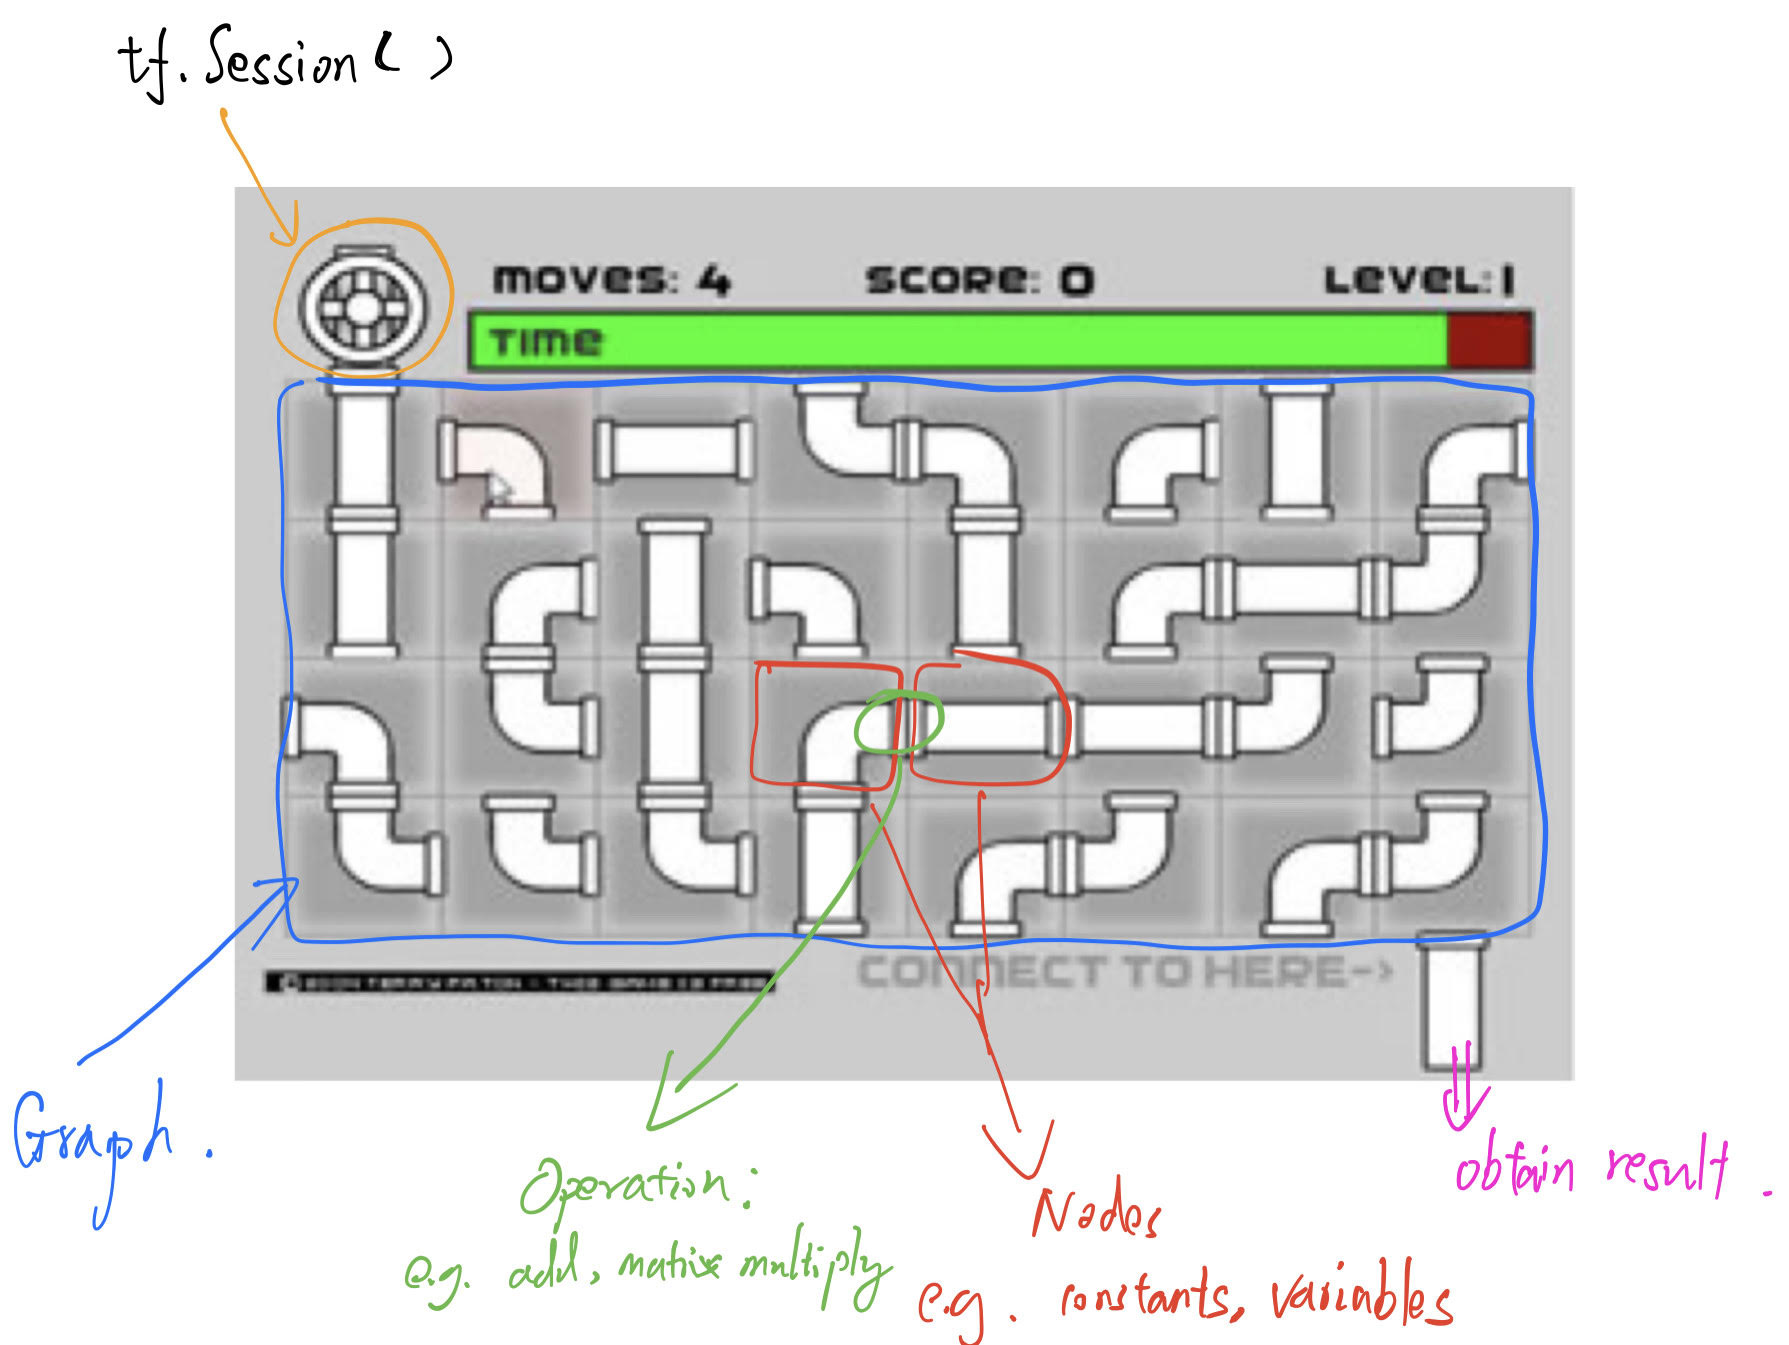
\includegraphics[width=9cm]{images/fig3.jpg}}
	\end{picture}
}
\end{frame}


\begin{frame}[fragile]{Tensorflow V1 versus V2}
\begin{itemize}
	\item V1: Nodes $ \to $  Operations $ \to$ Graph $\to$ Session $\to$ import the data
	\item V2: import the data $\to$ Nodes  $\to$ Operations (eager execution)
\end{itemize}
Pros and Cons:
\begin{itemize}
	\item V1 Pros: Integrity, a big picture of view
	\item V1 Cons: Lack of flexibility
	\item V2 Pros: Flexibility, you can always see the output step by step
	\item V2 Cons: Further efforts are frequently needed to pack the code up into a final package or class function
\end{itemize}
Therefore, V1 is frequently used in final delivery but V2 is good for debugging.
\end{frame}


\begin{frame}[fragile]{Tensorflow V1 versus V2}
Good news: V1 are V2 are both be accessible by tensorflow package.
\begin{itemize}
	\item Default is V2 (import tensorflow as tf)
	\item Use "import tensorflow.compat.v1 as tfv1" to call the functions and methods under V1
\end{itemize}
\end{frame}


\begin{frame}[fragile]{Basic widget: Constant}
The constant can be either scalar, vector, or matrix. It is just a concept which is opposite with variable. Variable can be changed in the future by using tf.assign() method, while the constant can not.
\begin{lstlisting}[style = Python]
s = tf.constant(2)
m = tf.constant([[1,2],[3,4]])
m = tf.constant([1,2,3,4],shape=[2,2])
\end{lstlisting}
With these two node, we can conduct a GRAPH and SESSION example. Here we use "tensorboard" for GRAPH and tf.Session() function for SESSION.
\end{frame}

\begin{frame}[fragile]{A simplest graph and session}
\begin{lstlisting}[style = Python]
g = tf.Graph()
with g.as_default():
    s = tf.constant(2)
    m = tf.constant([[1,2],[3,4]])
    mmul = s*m
g
\end{lstlisting}
Here, we have already completed a graph, to "open the faucet", we use tf.Session(), like:
\begin{lstlisting}[style = Python]
with tfv1.Session(graph=g) as sess:
    print(sess.run(mmul))
\end{lstlisting}
Finally, we get the result. Remark: The tf.Session() only exist in tensorflow v1, so we call this function under v1 platform.
\end{frame}

\begin{frame}[fragile]{Basic widget: Variable}
Variables are used to hold and update parameters. Another important difference with the constant is that it be treated as variable in the calculation of gradient. To create a variable, 
\begin{lstlisting}[style = Python]
w = tf.Variable(tf.ones((2,2))) # 2*2 matrix with all elements as 1
\end{lstlisting}
\begin{alertblock}{Alert}
The variable must be initialized immediately after "the data faucet is open" (i.e. tfv1.Session()).
\end{alertblock}
\begin{lstlisting}[style = Python]
with tfv1.Session() as sess:
    sess.run(tfv1.global_variables_initializer())
    print(sess.run(w))
\end{lstlisting}
\end{frame}

\begin{frame}[fragile]{Basic widget: Variable}
As we mentioned earlier, variable can be assigned with a new value. 
\begin{lstlisting}[style = Python]
with tfv1.Session() as sess:
    sess.run(tfv1.global_variables_initializer())
    print(sess.run(w))
    # Change w to a 2*2 matrix with all elements as 0
    sess.run(w.assign(tf.zeros((2,2)))) 
    print(sess.run(w))
\end{lstlisting}
\end{frame}


\begin{frame}[fragile]{Basic widget: Placeholder}
We can notice that although variable is more flexible than constant, it still need a initial value. In practice, sometimes the value of a parameter is determined by the actual data. So we need the placeholder to tell the PC, there is a variable, but I don't tell you the value, I will give you the value when I open the data faucet.
\begin{lstlisting}[style = Python]
import numpy as np
node1 = tfv1.placeholder(tf.float32,shape = [1,2])
node2 = tfv1.placeholder(tf.float32,shape = [1,2])
w_linear = tf.matmul(node1,w) + node2
with tfv1.Session() as sess:
    sess.run(tfv1.global_variables_initializer())
    print(sess.run(w))
    print(sess.run(w_linear,feed_dict={node1:np.matrix([1.0,2.0]),
    	node2:np.matrix([1.0,2.0])}))
\end{lstlisting}
\end{frame}

\begin{frame}[fragile]{Basic Operations}
Given $x$ and $y$,
\begin{itemize}
	\item x+y (element-wise): tf.add(x,y)
	\item x-y (element-wise): tf.subtract(x,y)
	\item x*y (element-wise): tf.multiply(x,y)
	\item x/y (element-wise): tf.divide(x,y)
	\item x*y (matrix style): tf.matmul(x,y)
	\item x<y (judgment): tf.less(x,y)
	\item x>y (judgment): tf.greater(x,y)
	\item x<=y (judgment): tf.less\_equal(x,y)
\end{itemize}
\end{frame}







\section{Neural Networks}

\begin{frame}[fragile]{ANN}
One of the greatest strengths of tensorflow is its ability to mimic learning and make predictions using data. This is done through structures known as Neural Networks. In the scope of this workshop, we're only covering Artificial Neural Networks known as ANNs.
\end{frame}

\begin{frame}[fragile]{ANNs Continued}
\begin{itemize}
	\item Approach like a black box with input and output
	\item Neurons
	\item Weights
\end{itemize}
\end{frame}


\section{Making our Model}

\begin{frame}[fragile]{NFL Play-By-Play Analysis}
Now it is time to create our Tensorflow Model! We're using play-by-play data from the NFL 2021-2022 season gathered from \href{http://nflsavant.com/about.php}{\tt \textcolor{blue}{NFLSavant}}. Let's try to create a model that predicts whether the next play is going to be a first down given data. 
\begin{center}
{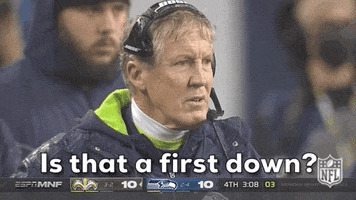
\includegraphics[width=8cm]{images/pete.jpg}}
\end{center}
\end{frame}


\section{Conclusion}

\begin{frame}{Takeaways}

\end{frame}

\begin{frame}{Shameless Promo}

Thank you very much for attending! The material for this workshop is accessible here --> \href{https://github.com/PranavTavildar1/Tensorflow-For-Sports-Analytics}{\tt \textcolor{blue}{Session Material}}.
\par
Join UConn Data Science Club! 
\par
Our UConntact --> \href{https://uconntact.uconn.edu/organization/datascience}{\tt \textcolor{blue}{Our UConntact}}.
\par
Our Discord --> \href{https://discord.gg/UJCZjXUWzg}{\tt \textcolor{blue}{Discord}}.

\end{frame}


\end{document}

